\section{Ergebnisse der Simulation}

Simulationen der Parkplatzsuche wurden durchgeführt. Dabei wurden verschiedene Parameter gespeichert. Somit standen nach den Simulationen Tabellen zur Verfügung, in denen die Parameter der Parkheuristik und die Position des gewählten Parkplatzes in Abhängigkeit der Zeit angegeben wurden. \\
Mit Hilfe dieser Tabellen wurden Graphen erzeugt, die vollständig im Anhang zu finden sind.\\
Innerhalb der Arbeit wird zu jeder Situation lediglich der Graph der Heuristik, die den besten Parkplatz, und die die den schlechtesten Parkplatz gewählt hat ausführlich betrachtet. Um die Güte des durchschnittlichen Parkplatzes zu bestimmen, wurde die lineare Approximation der Distanz betrachtet. \\
\subsection{Ein lernender Fahrer}\label{sec:sim_singlemutant}
\subsubsection{1 Auto pro Minute}
Bei diesem geringen Verkehrsaufkommen unterscheiden sich die Heuristiken in ihrer Güte kaum. Nahezu immer liegt der Parkplatz im Mittel zwischen 26 und 28.\\
Bei einem niedrigen Aufkommen an Autos findet die \emph{Block-Count}-Heuristik nach der oben beschriebenen Betrachtung die besten Parkplätze.
\begin{figure}
	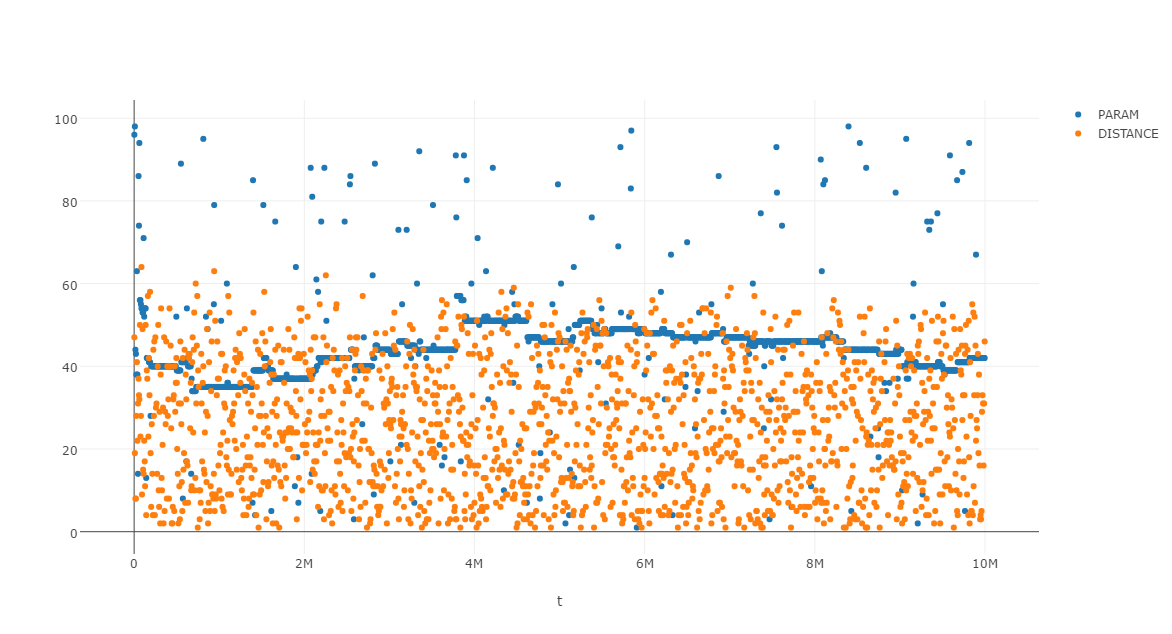
\includegraphics[width=\textwidth]{analyse/SingleMutant/blockcount1.png}
	\caption{Beste Heuristik bei einem lernenden Fahrer und einem Auto pro Minute: \emph{Block-Count}-Heuristik}\label{fig:res_sm_1pm_best}
\end{figure}
Hierbei wird der Parkplatz gewählt, der etwa 26  Plätze von der Destination entfernt ist. Dabei liegt der Parameterwert, also die Menge an direkt hintereinander geparkten Autos, an denen der lernende Fahrer vorbei fährt, bei etwa 43. Der Lernprozess dazu ist in Abbildung \ref{fig:res_sm_1pm_best} als Streudiagramm dargestellt.\\
Der schlechteste Parkplatz wird von der \emph{Car-Count}-Heuristik gewählt (siehe Abbildung \ref{fig:res_sm_1pm_worst}). 
\begin{figure}
	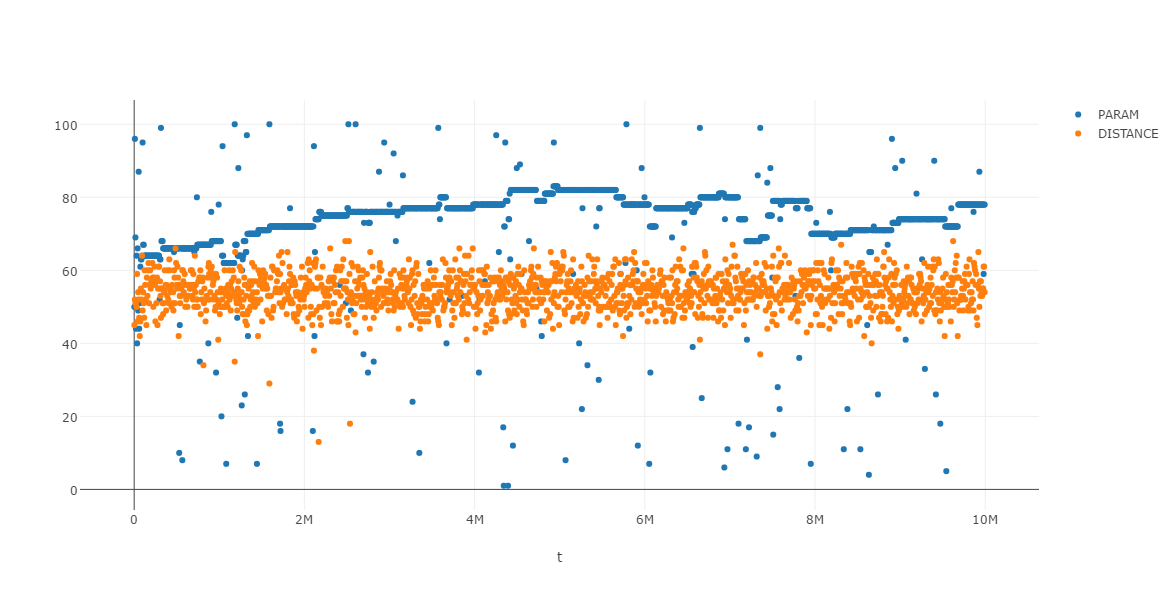
\includegraphics[width=\textwidth]{analyse/SingleMutant/carcount1.png}
	\caption{Schlechteste Heuristik bei einem lernenden Fahrer und einem Auto pro Minute: \emph{Car-Count}-Heuristik}\label{fig:res_sm_1pm_worst}
\end{figure}
Dieser ist sogar mehr als doppelt so weit von der Destination entfernt (54).
Hierbei lernt der Fahrer an etwa 75 geparkten Autos vorbei zu fahren, bevor er den nächsten freien Parkplatz wählt.\\
Man sieht an den Graphen, dass es zwar im Durchschnitt sinnvoll ist, Blöcke zu zählen, Autos zu zählen führt jedoch zu einer stabileren Verteilung.\\
Somit ist der Parkplatz im Mittel zwar wesentlich schlechter, jedoch ist es nahezu garantiert, dass man nie wesentlich schlechter parkt.

\subsubsection{2 Autos pro Minute}

Verändert sich das Verkehrsaufgebot, so werden Unterschiede in den Erfolgen der Heuristiken deutlicher.\\
Auch bei mittlerem Verkehrsaufkommen erscheint es sinnvoll, die \emph{Block-Count}-Heuristik anzuwenden, denn auch hier findet diese im Schnitt die besten Parkplätze. 
\begin{figure}
	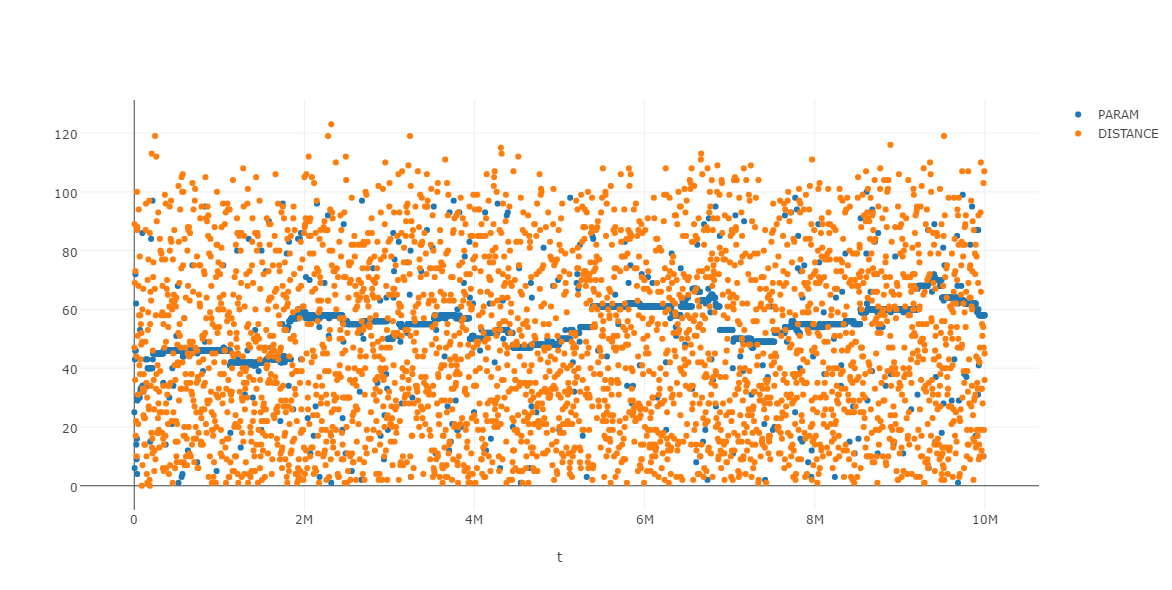
\includegraphics[width=\textwidth]{analyse/SingleMutant/blockcount2.png}
	\caption{Beste Heuristik bei einem lernenden Fahrer und zwei Autos pro Minute: \emph{Block-Count}-Heuristik}\label{fig:res_sm_2pm_best}
\end{figure}
Aufgrund dessen, dass mehr Parkplätze belegt werden, entfernt sich der mittlere Parkplatz von der Destination, im Vergleich zum mittleren Parkplatz, wenn lediglich ein Auto pro Minute auf den Parkplatz fährt.\\
Mit der \emph{Block-Count}-Heuristik wird nun ein Platz gewählt, der etwa 46 Plätze vom Ziel entfernt ist. Wobei der lernende Fahrer beschließt an 62 hintereinander geparkten Autos vorbei zu fahren um danach einen Parkplatz zu finden. Dabei ist die Näherungsgerade jedoch steigend, was bedeutet, der Fahrer würde bei weiteren Wiederholungen weiter lernen und möglicherweise an mehr geparkten Autos vorbei fahren (siehe Abbildung \ref{fig:res_sm_2pm_best}).\\
Der im Schnitt schlechteste Parkplatz wird in diesem Fall bei der  \emph{X-Out-Of-Y}-Heuristik gewählt. \\
\begin{figure}
	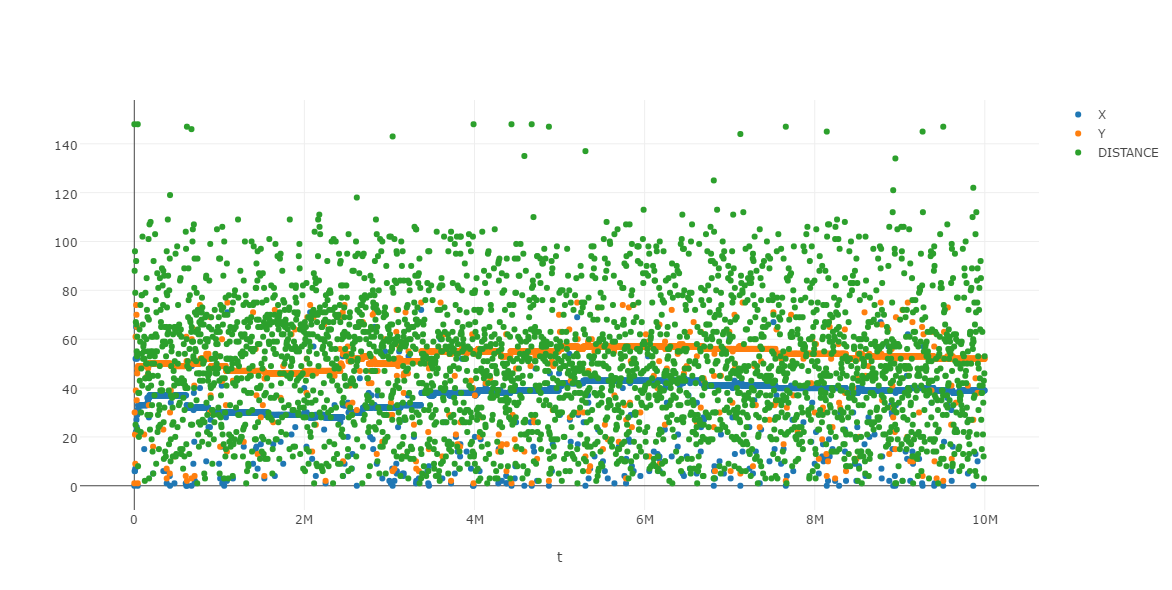
\includegraphics[width=\textwidth]{analyse/SingleMutant/xy2.png}
	\caption{Schlechteste Heuristik bei einem lernenden Fahrer und zwei Autos pro Minute: \emph{X-Out-Of-Y}-Heuristik}\label{fig:res_sm_2pm_worst}
\end{figure}
Dabei beträgt der Abstand zum Ziel etwa 53 Plätze. Dieser wird dadurch gefunden, dass der Fahrer einen Parkplatz wählt, sobald er an einem Block von 53 Parkplätzen vorbeigefahren ist, von denen 40 besetzt waren (siehe Abbildung \ref{fig:res_sm_2pm_worst}).\\
Hier hätte man erwarten können, dass $X$ und $Y$ sich annähern, da bei $X=Y$ die block count Heuristik erreicht wird. Man stellt jedoch fest, dass in diesem Fall der Abstand zwischen $X$ und $Y$ relativ stabil bei 13 bleibt.\\
Zusätzlich zeigt dieses Kapitel, dass es durchaus sinnvoll ist, verschiedene Dichten an ankommenden Autos zu betrachten, so ist die \emph{Car-Count}-Heuristik nicht nur als schlechteste Heuristik ersetzt worden, man sieht sogar, dass dieses die einzige Heuristik ist, bei der sich der mittlere Parkplatz nicht verschlechtert. Es wird dort sogar nur noch 53 Plätze vom Ziel entfernt geparkt (siehe Abbildung \ref{fig:ap_sm_cc_2}).

\subsubsection{4 Autos pro Minute} 

In diesem Fall ändert sich nichts daran, welche Heuristik am besten und welche am schlechtesten abschneidet.\\
Bei der Block count Heuristik wird nun ein Platz gewählt, der etwa 63 Plätze vom Ziel entfernt ist und bei x out of y ist er etwa 74 Plätze vom Ziel entfernt. \\
\begin{figure}
	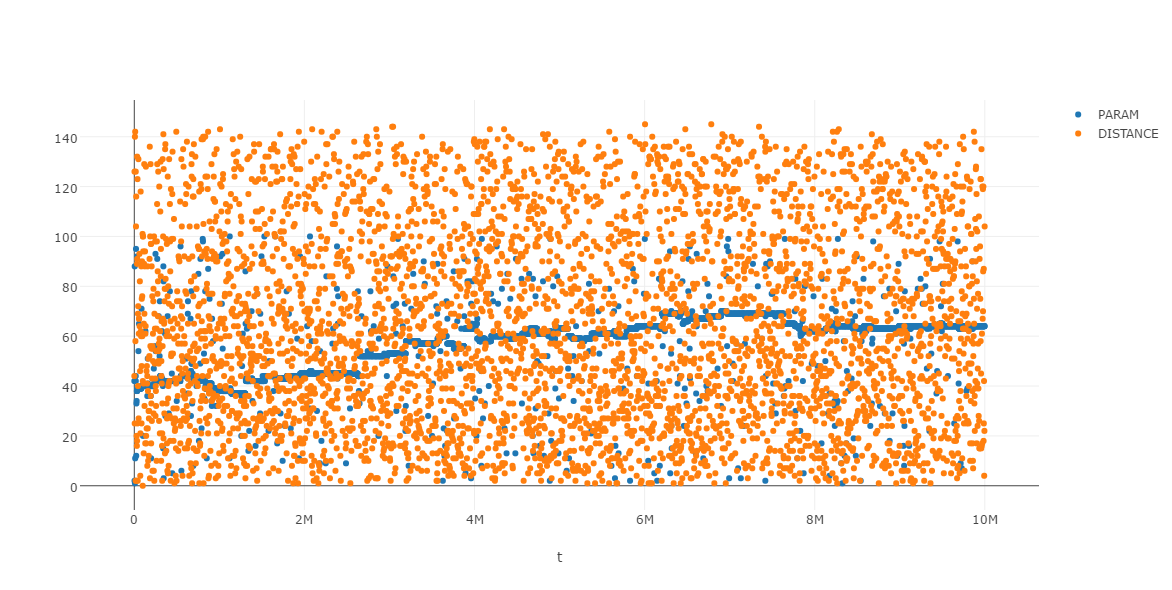
\includegraphics[width=\textwidth]{analyse/SingleMutant/blockcount4.png}
	\caption{Beste Heuristik bei einem lernenden Fahrer und vier Autos pro Minute: \emph{Block-Count}-Heuristik}\label{fig:res_sm_4pm_best}
\end{figure}
\begin{figure}
	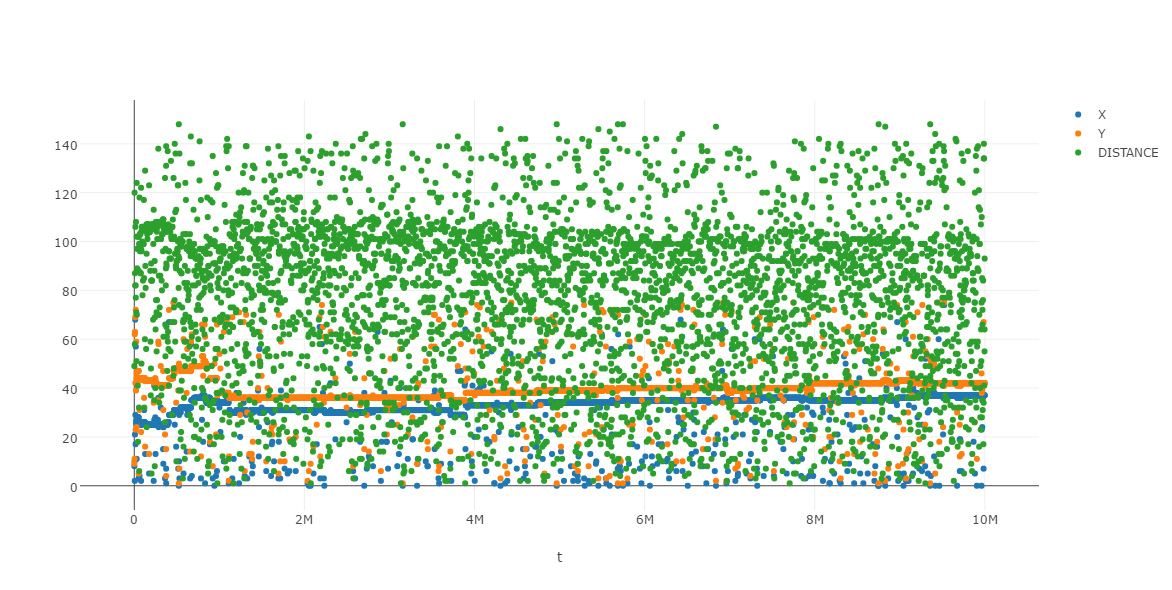
\includegraphics[width=\textwidth]{analyse/SingleMutant/xy4.png}
	\caption{Schlechteste Heuristik bei einem lernenden Fahrer und vier Auto pro Minute: \emph{X-Out-Of-Y}-Heuristik}\label{fig:res_sm_4pm_worst}
\end{figure}
Während hier jedoch bei der \emph{Block-Count}-Heuristik die Approximationsgerade der Abstände zum Ziel nahezu parallel zur $t$-Achse ist, ist sie bei \emph{X-Out-Of-Y}-Heuristik fallend. Dies ist bei den beiden schlechtesten Heuristiken so. Auch die \emph{Fixed-Distance}-Heuristik findet derzeit einen Parkplatz der etwa 68 Plätze von der Destination entfernt ist, hat sich jedoch im Verlauf der Simulation signifikant verbessert.\\
Ebenso fällt auf, dass der Abstand von X zu Y etwas verkleinert wurde. Dieser beträgt nun lediglich noch 5, wobei auch die Blöcke verkleinert wurden. Hier müssen nun noch 37 von 42 Plätzen belegt sein, um danach einen Parkplatz zu wählen.\\
Der Parameter der Block count Heuristik hat sich nahezu nicht mehr verändert und liegt nun bei 63.\\

Würden also alle Anderen zufällig einen Parkplatz auswählen und nur man selbst würde lernen, so wäre es bei jedem Verkehrsaufkommen optimal die \emph{Block-Count}-Heuristik anzuwenden und lediglich die Blocklänge an das Verkehrsaufkommen anzupassen. 

\subsection{Mehrere lernende Fahrer}

Für dieses Kapitel wurde die Simulation erneut durchgeführt, wobei in jedem Durchlauf jede Heuristik von einigen Fahrern verfolgt wird. \\
Auch hier wurde untersucht welche Heuristik den besten Parkplatz für ein bestimmtes Verkehrsaufkommen findet.

\subsubsection{1 Auto pro Minute}\label{sec:sim_pm_1pm}

Wenn einige Fahrer gezielt einen Parkplatz suchen, finden die gleichen Heuristiken den besten und den schlechtesten mittleren Parkplatz wie in der in Abschnitt \ref{sec:sim_singlemutant} betrachteten Simulation. 
\begin{figure}
	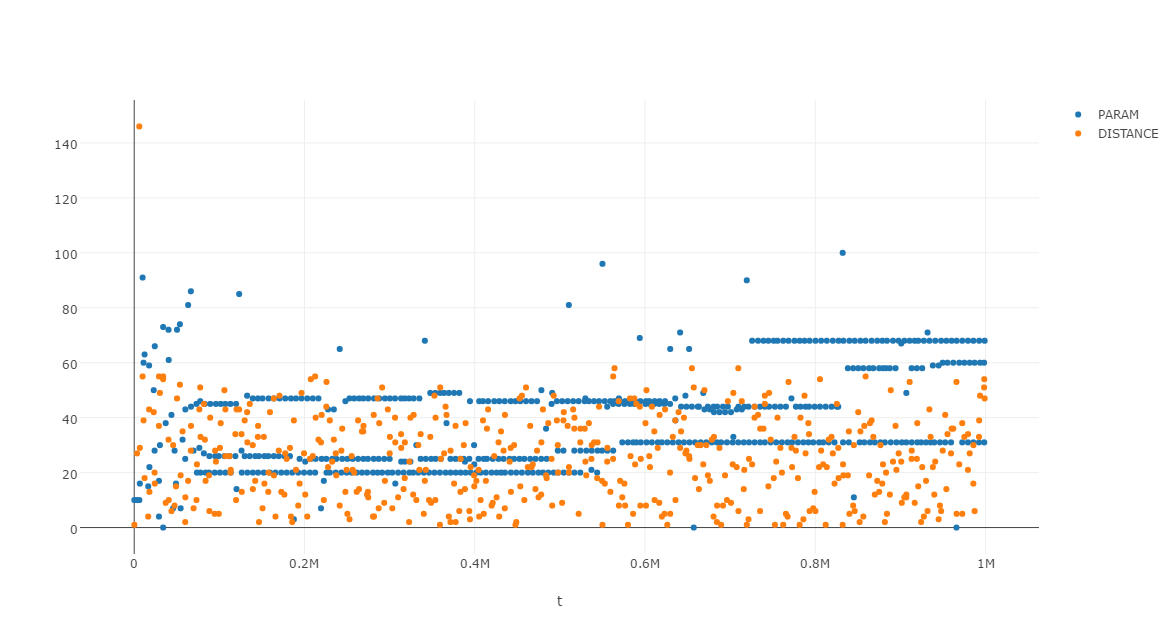
\includegraphics[width=\textwidth]{analyse/SomeMutants/1pm/block1some.png}
	\caption{Beste Heuristik bei mehreren lernenden Fahrern und einem Auto pro Minute: \emph{Block-Count}-Heuristik}\label{fig:res_pm_1pm_best}
\end{figure}
In diesem Fall wird am Ende der Simulation ein Parkplatz gefunden der im Schnitt 23 Plätze von der Destination entfernt ist (Abbildung \ref{fig:res_pm_1pm_best}).\\
Um die Realität möglichst genau abzubilden lernt jeder Autofahrer ,,für sich selbst''. Ein Informationsaustausch zwischen Fahrern mit der gleichen Heuristik findet nicht statt, was in der Realität auch eher unwahrscheinlich wäre. Die individuellen Parameter sind in den Abbildungen an den parallelen Parameterverläufen ablesbar. Es bliebe noch zu untersuchen, wie sich der mittlere Parkplatz verändern würde, wenn ein mittlerer Parameter, der in diesem Fall am Ende bei 51 liegt, von allen uniform gewählt werden würde.\\

Die \emph{Car-Count}-Heuristik findet wieder den mit Abstand schlechtesten mittleren Parkplatz. Dieser ist sogar noch etwas schlechter als im ersten Durchlauf (Abbildung \ref{fig:res_pm_1pm_worst}).\\
\begin{figure}
	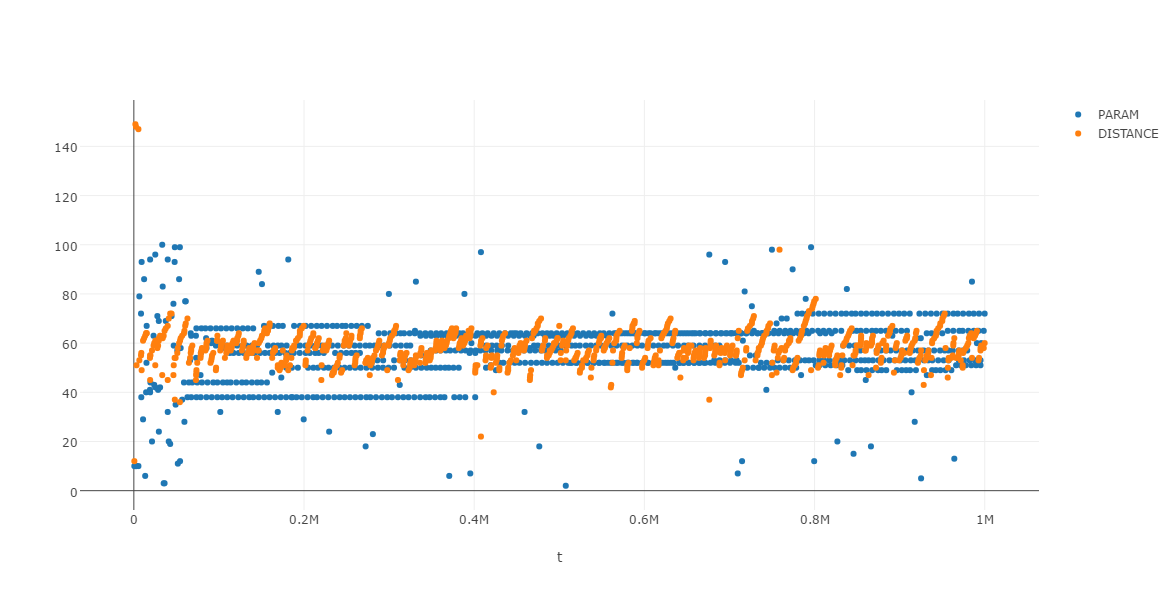
\includegraphics[width=\textwidth]{analyse/SomeMutants/1pm/car1some.png}
	\caption{Schlechteste Heuristik bei mehreren lernenden Fahrern und einem Auto pro Minute: \emph{Car-Count}-Heuristik}\label{fig:res_pm_1pm_worst}
\end{figure}
Dabei wird nach durchschnittlich nach 61 geparkten Autos ein Parkplatz gewählt, der dann im Schnitt 58 Plätze von der Destination entfernt ist.\\

Es wurde bei der Untersuchung deutlich, dass der Lernalgorithmus besser funktioniert als im ersten Durchlauf. Dies kann daran liegen, dass durch die Erhöhung der Lerner-Anzahl der Effekt des Lernens verstärkt wird.\\
Am Ende der Simulation werden bei nahezu allen Heuristiken Plätze gewählt die wesentlich besser sind, als zu Beginn.

\subsubsection{2 Autos pro Minute}\label{sec:sim_partmutant_2pm}

Erhöht sich die Anzahl der ankommenden Autos so bleibt die \emph{Car-Count}-Heuristik weiterhin die Schlechteste (Abbildung \ref{fig:res_pm_2pm_worst}). 
\begin{figure}
	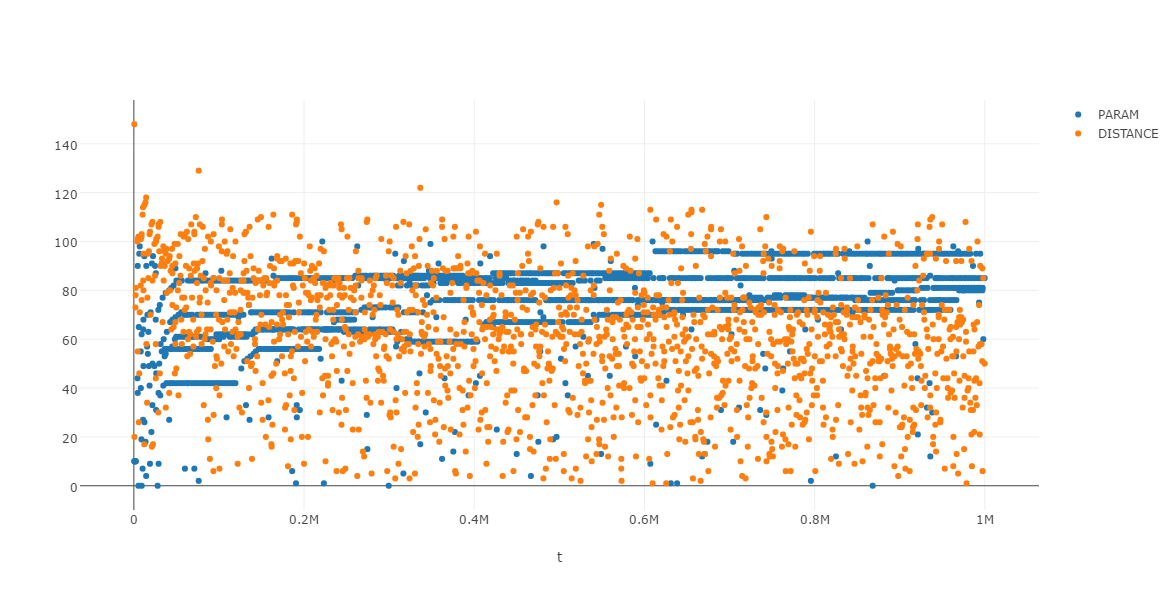
\includegraphics[width=\textwidth]{analyse/SomeMutants/2pm/car2some.png}
	\caption{Schlechteste Heuristik bei mehreren lernenden Fahrern und zwei Autos pro Minute: \emph{Car-Count}-Heuristik}\label{fig:res_pm_2pm_worst}
\end{figure}
Hier wird am Ende der Simulation ein Parkplatz gewählt, der 50 Plätze von der Destination entfernt ist. Dafür werden im Schnitt 85 Autos passiert.\\
Es zeigt sich jedoch auch, dass innerhalb dieser Heuristik der mittlere Parkplatz am Stärksten verbessert wird.\\
Die Parkplätze die am Anfang der Simulation gewählt werden liegen 73 Plätze vom Ziel entfernt. Zusätzlich ist dies die einzige Heuristik, bei der bei diesem höheren Verkehrsaufkommen ein besserer Parkplatz gewählt wird. Dies wurde bereits im ersten Durchlauf festgestellt.\\
Der beste Parkplatz wird hier durch die \emph{X-Out-Of-Y}-Heuristik gefunden.\\
\begin{figure}
	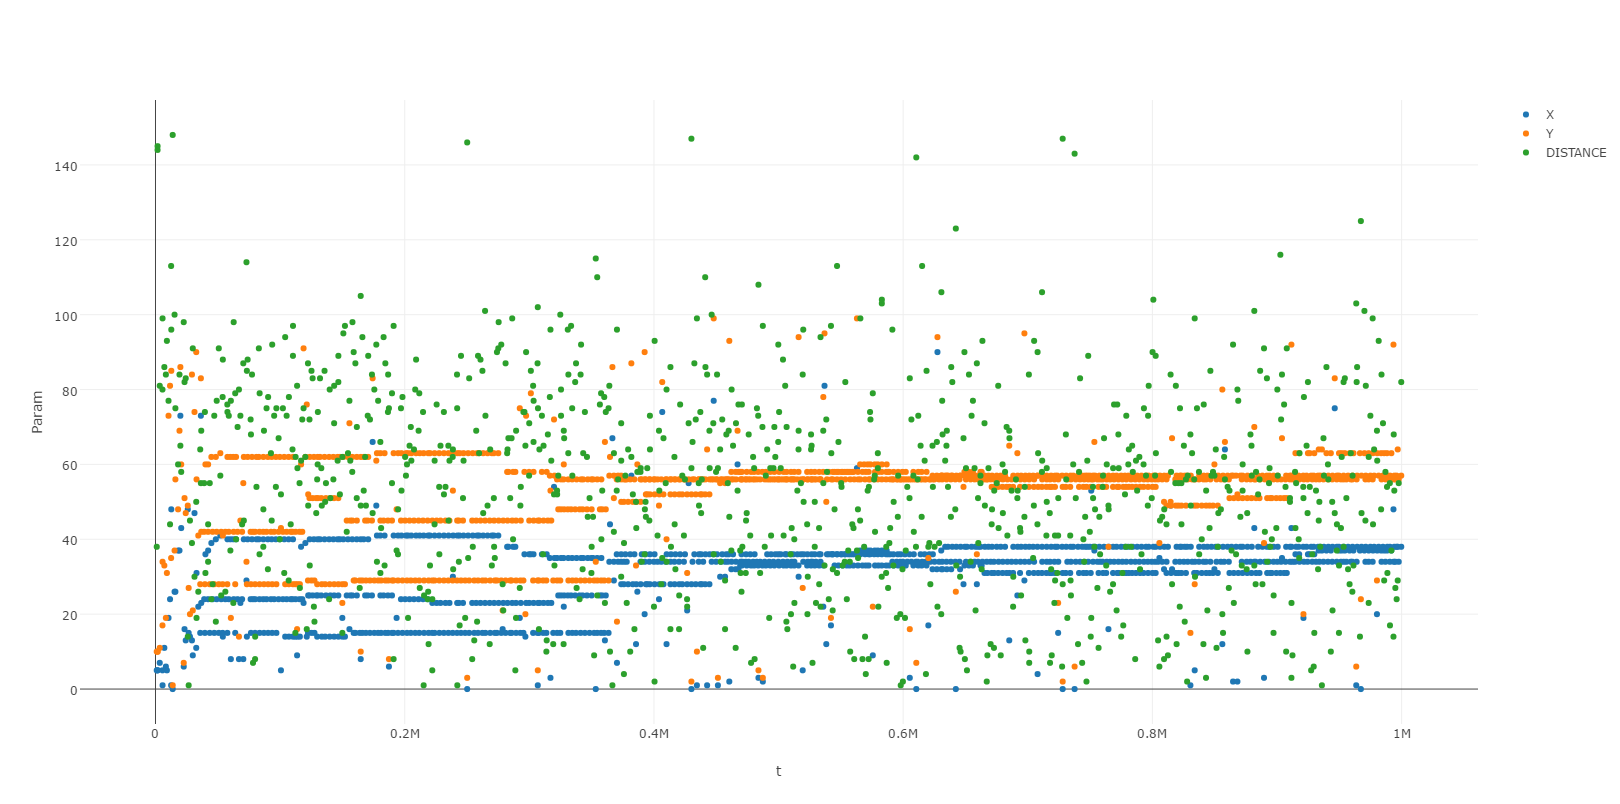
\includegraphics[width=\textwidth]{analyse/SomeMutants/2pm/xy.png}
	\caption{Beste Heuristik bei mehreren lernenden Fahrern und zwei Autos pro Minute: \emph{X-Out-Of-Y}-Heuristik}\label{fig:res_pm_2pm_best}
\end{figure}
Hierbei wird ein Parkplatz gefunden, der 46 Plätze entfernt ist. Dabei wird im Schnitt ein Platz gewählt, wenn von den letzten 59 Plätzen 37 besetzt waren (Abbildung \ref{fig:res_pm_2pm_best}).

\subsubsection{4 Autos pro Minute}

Auch bei hohem Verkehrsaufkommen findet die \emph{Car-Count}-Heuristik den Schlechtesten mittleren Parkplatz. \\
\begin{figure}
	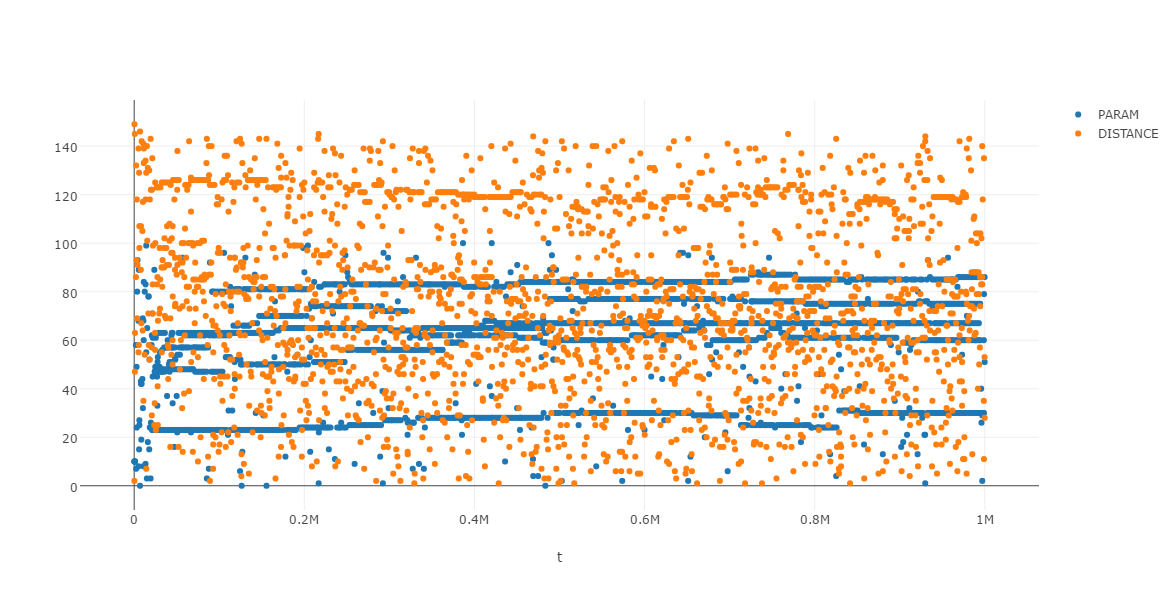
\includegraphics[width=\textwidth]{analyse/SomeMutants/4pm/car4some.png}
	\caption{Schlechteste Heuristik bei mehreren lernenden Fahrern und vier Autos pro Minute: \emph{Car-Count}-Heuristik}\label{fig:res_pm_4pm_worst}
\end{figure}
Nach der Beobachtung in Abschnitt \ref{sec:sim_partmutant_2pm} hätte man zu dem Schluss kommen können, dass eine höhere Fahrerdichte dazu führt dass diese Heuristik immer besser wird. Sie findet nun jedoch wieder einen Platz, der schlechter ist als zuvor. Etwa 71 Plätze vom Ziel entfernt findet sie im Mittel einen Parkplatz und fährt dafür an 65 geparkten Autos vorbei (Abbildung \ref{fig:res_pm_4pm_worst}).\\
Die \emph{Fixed-Distance}-Heuristik findet hier wiederum den besten Parkplatz. 
\begin{figure}
	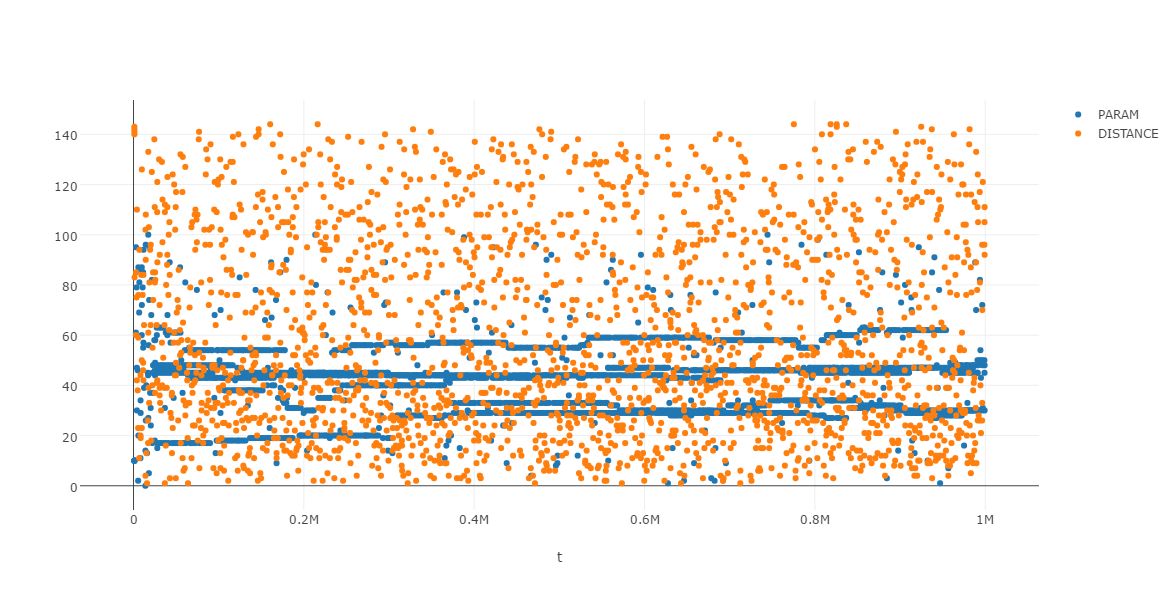
\includegraphics[width=\textwidth]{analyse/SomeMutants/4pm/fixed4some.png}
	\caption{Beste Heuristik bei mehreren lernenden Fahrern und vier Autos pro Minute: \emph{Fixed-Distance}-Heuristik}\label{fig:res_pm_4pm_best}
\end{figure}
Der Platz liegt etwa durchschnittlich 59 Plätze vom Ziel entfernt, während der mittlere Fahrer auf 43 Plätze an das Ziel heran fährt (Abbildung \ref{fig:res_pm_4pm_best}). Dadurch, dass der letztendliche Abstand höher ist, als die fixierte Distanz, kann man schließen dass der Fahrer am Ende des Platzes wenden muss, um auf dem Rückweg den ersten Platz zu wählen.\\
  Daher bekommt man zwar den besten Parkplatz, aber ob die Heuristik dann als ,,gut'' einzuschätzen ist, ist fraglich. Es scheint eher sinnvoll zu sein, an allen Parkplätzen vorbeizufahren und nach dem Wenden den ersten Platz zu wählen. \\
  
	\subsubsection{Hypothese}\label{sec:sim_hypo}  
  
  Im Gegensatz zur ersten Untersuchung hat sich nun also gezeigt, dass es in dieser Situation sinnvoll ist, seine Heuristik an das Verkehrsaufkommen anzupassen und nicht lediglich die Parameter zu verändern.\\
  Außerdem hat sich gezeigt, dass für jede Dichte ein besserer Platz gefunden wird, wenn mehrere Fahrer lernen. Daher könnte man vermuten, dass es sinnvoll ist, Fahrern beizubringen wie sie gezielt Parkplätze finden. Ob diese Hypothese realistisch ist, kann nun in der nächsten Simulation überprüft werden. 
  
  \subsection{Alle Fahrer lernen}
  
Auch hier treten in jedem Durchlauf alle Heuristiken gegeneinander an. Werden jetzt jedoch schlechtere Parkplätze gefunden, als im letzten Durchlauf, so ist die in Abschnitt \ref{sec:sim_hypo} aufgestellte Hypothese widerlegt.

  \subsubsection{1 Auto pro Minute}
  
Wie auch in den vorherigen Beispielen findet auch hier die Car count Heuristik den mit Abstand schlechtesten mittleren Parkplatz. 
\begin{figure}
	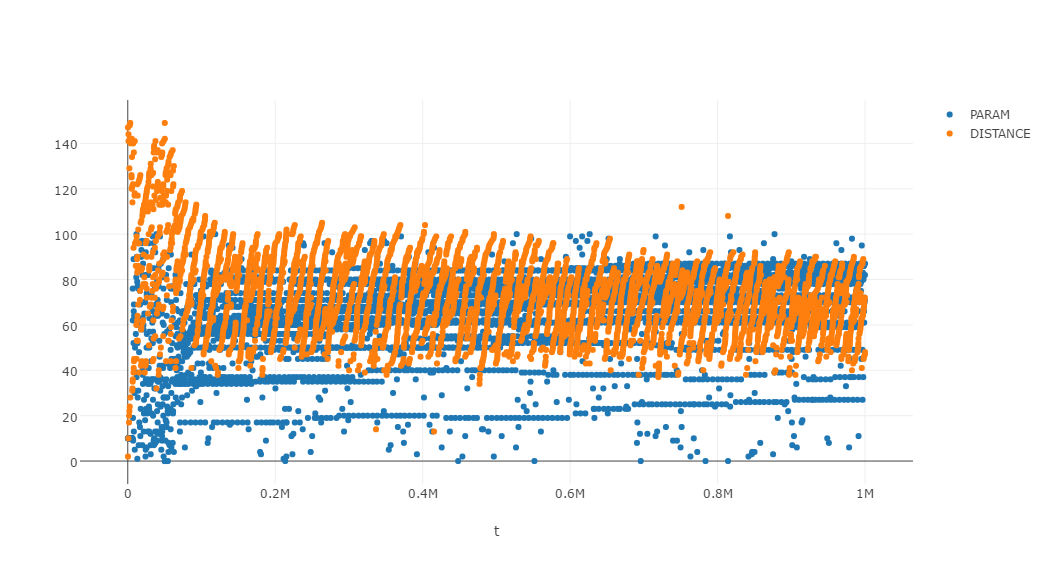
\includegraphics[width=\textwidth]{analyse/JustHeuristik/1pm/car1just.png}
	\caption{Schlechteste Heuristik bei nur lernenden Fahrern und einem Auto pro Minute: \emph{Car-Count}-Heuristik}\label{fig:res_jh_1pm_worst}
\end{figure}
Dieser ist wieder schlechter als in der Simulation aus Abschnitt \ref{sec:sim_pm_1pm}. Diesmal wird durchschnittlich 63 Plätze vom Ziel entfernt geparkt (Abbildung \ref{fig:res_jh_1pm_worst}). Diese Heuristik unterscheidet sich in mehreren Merkmalen signifikant von den Anderen. Sie verbessert sich nicht nur beim Übergang von der geringen zur mittleren Dichte, sondern verschlechtert sich auch, je mehr Fahrer gezielt einen Parkplatz wählen.\\
In dieser Simulation wird der beste Platz wieder von der \emph{X-Out-Of-Y}-Heuristik gewählt. 
\begin{figure}
	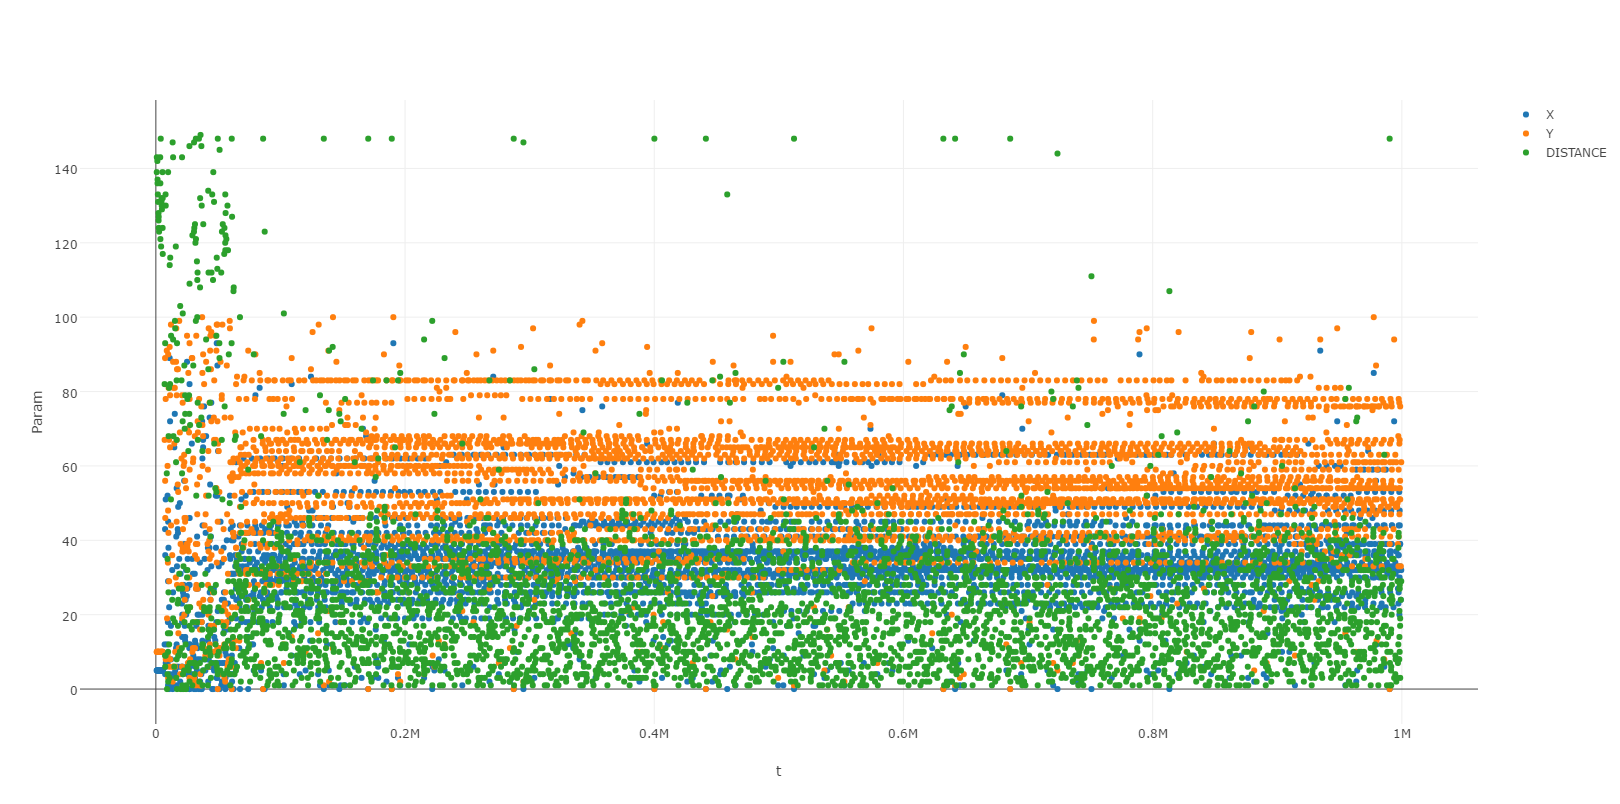
\includegraphics[width=\textwidth]{analyse/JustHeuristik/1pm/xy.png}
	\caption{Beste Heuristik bei nur lernenden Fahrern und zwei Autos pro Minute: \emph{X-Out-Of-Y}-Heuristik}\label{fig:res_jh_1pm_best}
\end{figure}
Wenn von 58 Plätzen 37 besetzt sind wird ein Platz gewählt, der etwa 17 Plätze vom Ziel entfernt ist (Abbildung \ref{fig:res_jh_1pm_best}). \\
Der beste Parkplatz der gefunden wird ist also besser als in den vorherigen Beispiel, womit die Hypothese nicht widerlegt werden konnte.\\

\subsubsection{2 Autos pro Minute}

Wie es zu erwarten war, hat sich die \emph{Car-Count}-Heuristik verbessert, bleibt jedoch weiterhin die Schlechteste.\\
Nachdem 78 Autos passiert wurden wird ein Platz gewählt, der 55 Plätze vom Ziel entfernt ist (Abbildung \ref{fig:ap_jh_cc_2} im Anhang).\\
Die Heuristik mit dem linearen Operator findet den besten Platz. 
\begin{figure}
	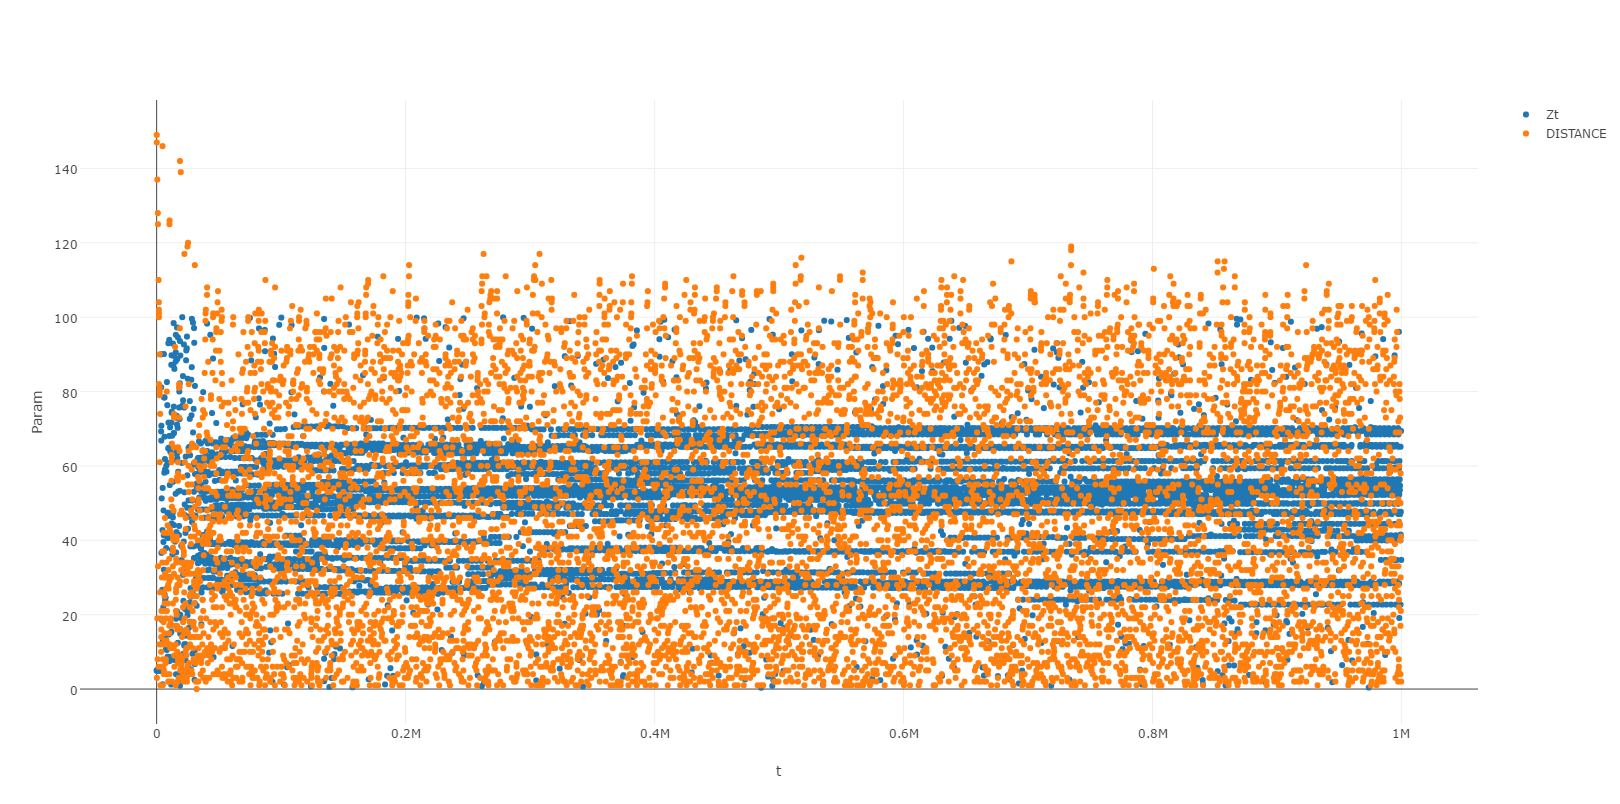
\includegraphics[width=\textwidth]{analyse/JustHeuristik/2pm/linop.png}
	\caption{Beste Heuristik bei nur lernenden Fahrern und zwei Autos pro Minute: \emph{Linear-Operator}-Heuristik Dargestellt ist nur der Schrankenparameter $z_T$. Die Geschwindigkeit ist in Abbildung \ref{fig:ap_jh_loa_2} zu finden.} \label{fig:res_jh_2pm_best}
\end{figure}
Mit den gelernten Parametern kann die Ungleichung 
\begin{align}
0,49\cdot z_i+b_i > 51
\end{align} aufgestellt werden. Sobald diese für einen freien Parkplatz erfüllt ist, wird dieser gewählt und ist, in der Simulation, etwa 35 Plätze von der Destination entfernt (Abbildung \ref{fig:res_jh_2pm_best}).\\
Somit ist die Hypothese weiterhin nicht falsifiziert. Es ist jedoch fraglich, ob der lineare Operator in der Realität anwendbar ist. \\

\subsubsection{4 Autos pro Minute}

Wie im letzten Unterkapitel findet auch hier die \emph{Fixed-Distance}-Heuristik den besten Parkplatz.
\begin{figure}
	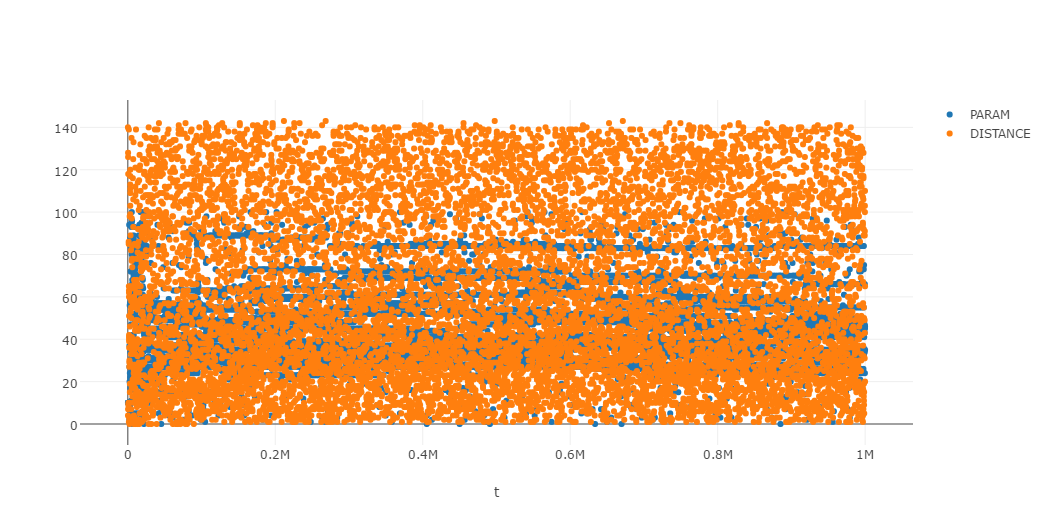
\includegraphics[width=\textwidth]{analyse/JustHeuristik/4pm/fixed4just.png}
	\caption{Beste Heuristik bei nur lernenden Fahrern und zwei Autos pro Minute: \emph{Fixed-Distance}-Heuristik} \label{fig:res_jh_4pm_best}
\end{figure}
Es ist jedoch wieder so, dass der Fahrer auf 46 Plätze an das Ziel heran fährt und einen Platz erhält, der 62 Plätze vom Ziel entfernt ist (Abbildung \ref{fig:res_jh_4pm_best}). Die Platzwahl verschlechtert sich sogar im Verlauf der Simulation. Zu Beginn ist der Platz lediglich 61 Plätze entfernt.\\
Die schlechtesten Plätze werden vom linearen Operator und der \emph{Space-Count}-Heuristik gefunden. Nachdem ein Fahrer an 46 freien Plätzen vorbeigefahren ist, wählt er einen Platz der im Schnitt 69 Plätze vom Ziel entfernt ist (Abbildungen \ref{fig:ap_jh_loz_4}, \ref{fig:ap_jh_loa_4} \& \ref{fig:ap_jh_sc_4} im Anhang).\\

Der beste Platz der hier gewählt wird ist also etwas schlechter, als im Fall von wenigen Lernenden. Jedoch wurde in diesen Fällen der im Mittel beste Platz auch nicht von einer optimierten Heuristik gefunden, sondern durch Wenden und das Wählen eines Platzes auf dem Rückweg!\\
Für die niedrige und mittlere Dichte konnte die Hypothese nicht widerlegt werden. Bei hohen Verkehrsaufkommen müssten weitere Untersuchungen angestellt werden.

\subsection{Zusammenfassung}

Vorläufig lässt sich sagen, dass kein Fahrer zufällig einen Parkplatz wählen sollte. Demnach sollten Fahrschüler Heuristiken lernen. Falls spätere Untersuchungen zeigen, dass es sinnvoll ist, wenn alle die gleiche Heuristik nutzen und dort einen mittleren Wert für die Parameter wählen, können auch diese Informationen in der Fahrschule vermittelt werden.\\
Am wahrscheinlichsten scheint es derzeit zu sein, davon auszugehen, dass einige, aber nicht alle Fahrer systematisch einen Parkplatz wählen. \\
 Dann kann man Fahrern raten bei niedrigem Verkehrsaufkommen die \emph{Block-Count}-Heuristik zu verfolgen. Dabei kann mit einem Block von 51 Autos gestartet werden und dieser Parameter durch Variation verbessert werden.\\
 Kommen etwa 2 Autos pro Minute auf dem Parkplatz an, so ist es sinnvoll diese Heuristik leicht zu verändern und die \emph{X-out-Of-Y}-Heuristik zu verwenden. Dabei kann mit Blöcken von 59 Plätzen von denen 37 belegt sind gestartet werden.\\
 Bei hohem Betrieb auf dem Platz scheint es am Besten zu sein, den kompletten Parkplatz zu passieren und auf dem Rückweg den ersten Platz zu wählen.\\
All diese Erkenntnisse sind jedoch sehr theoretischer Natur und bedürfen praktischen Projekten zur Überprüfung und darauf basierenden Überarbeitungen der Simulation. 
 
 \subsection{Ausblick}

Es hat sich herausgestellt, dass es sinnvoll ist, wenn alle Fahrer gezielt nach Parkplätzen suchen, wobei dies für eine hohe Dichte weiterer Untersuchungen bedarf. Da jedoch ein Austausch über die gewählten Parameter sehr unwahrscheinlich ist, sollte noch untersucht werden, wie sich die Wahl eines Mittelwertes als Parameter für alle auswirkt.\\
Zusätzlich fand keine Untersuchung darüber statt, wie es sich verhält, wenn alle lernenden Fahrer die gleiche Heuristik verwenden. Würde dies jedoch untersucht werden, so könnten am effizientesten Anweisungen an Fahrer weitergegeben werden. \\
Außerdem wäre sie Untersuchung realer Parkplätze möglich, um für einen real existierenden Parkplatz Strategien zu testen.\\
All diese Untersuchungen sind nicht nur mathematisch interessant. Durch die erhöhte Wahrscheinlichkeit einen guten Parkplatz zu finden wird das Wohlbefinden der Autofahrer gestärkt, wodurch sie sich möglicherweise länger in einem Kaufhaus oder Restaurant aufhalten und dort mehr Geld ausgeben. Zusätzlich tritt bei der Parkplatzsuche weniger Stress auf, wodurch eventuell die Unfallwahrscheinlichkeit gesenkt werden kann.